\documentclass[main.tex]{subfiles} % Subfile-Class

% ============================================================================== %
%                            Subfile document                                    %
% ============================================================================== %

\begin{document}

% Template

\subsection{Produktbeschreibung}

Das in diesem Projekt entwickelte System ist ein autonomes Fahrzeug, das in der
Lage ist, sich selbstständig durch ein Wegenetzwerk zu navigieren. Es wurde
speziell für die Aufgabe konzipiert, dynamisch auf Hindernisse und
Einschränkungen zu reagieren, um den optimalen Weg von einem definierten
Startpunkt zu einem Zielpunkt zu finden.

Das Fahrzeug zeichnet sich durch eine modulare Bauweise aus, die es ermöglicht,
verschiedene Technologien effizient zu integrieren. Zu den zentralen
Komponenten gehören:

\begin{itemize}
    \item \textbf{Chassis und Antrieb:} Das Fahrzeug verwendet ein leichtes, stabiles Chassis, das auf einem dreirädrigen Konzept basiert. Zwei Antriebsräder sorgen für die Fortbewegung, während ein stabilisierender Auflagepunkt zusätzliche Balance bietet. Die Antriebssteuerung erfolgt über Schrittmotoren, die eine präzise Bewegung und Manövrierfähigkeit gewährleisten.

    \item \textbf{Sensorik:} Ein Set aus Liniensensor, Kamera, Ultraschallsensor, Lichtschranke und einem LiDAR-System ermöglicht es dem Fahrzeug, die Umgebung präzise zu analysieren. Der Liniensensor dient ausschliesslich der Verfolgung von Leitlinien. Schranken werden mithilfe von Ultraschallsensoren und/oder Lichtschranken erkannt, während LiDAR auf einer spezifischen Höhe dazu eingesetzt wird, Pylonen (gesperrte Wegpunkte) zu identifizieren. Die Kamera wird ausschliesslich dafür genutzt, Knotenpunkte frühzeitig zu erkennen, bevor sie überfahren werden, sowie Zielknoten eindeutig zu identifizieren. Diese Sensoren arbeiten zusammen, um eine Echtzeitbewertung der Umgebung durchzuführen.

    \item \textbf{Steuerungseinheit:} Ein Mikrocontroller-basiertes System übernimmt die Verarbeitung der Sensordaten und die Steuerung der Motoren. Durch die Integration eines speziell entwickelten Algorithmus wird das Fahrzeug in die Lage versetzt, dynamisch auf Veränderungen der Umgebung zu reagieren.

    \item \textbf{Greifeinheit:} Für das Entfernen von Hindernissen ist das Fahrzeug mit einem motorisierten Greifer ausgestattet. Dieser kann Objekte sicher greifen, anheben und präzise zurücklegen.

    \item \textbf{Energieversorgung:} Das System wird durch einen kompakten Lithium-Polymer-Akku betrieben, der eine ausreichende Betriebsdauer für die vorgegebene Aufgabenstellung sicherstellt. Zusätzliche Sicherheitsfunktionen wie eine Überwachung der Zellspannung und ein Not-Aus-Knopf garantieren die Betriebssicherheit.

    \item \textbf{Benutzerinterface:} Über einen Wahlschalter kann vor dem Start die Zielposition ausgewählt werden. Visuelle und akustische Signale zeigen den Abschluss der Aufgabe an.

    \item \textbf{Simulator:} Zur Unterstützung der Entwicklung und zur frühzeitigen Validierung von Algorithmen hat das Informatik-Team einen Simulator in \textit{Svelte.js} entwickelt. Der Simulator ermöglicht es, das Verhalten des Fahrzeugs in einer virtuellen Umgebung zu testen, bevor physische Prototypen gebaut werden. Mit Funktionen wie der Simulation von Hindernissen, gesperrten Wegpunkten und alternativen Routen erlaubt der Simulator eine präzise Analyse der Navigations- und Steuerungsalgorithmen. Zudem bietet das Tool eine interaktive Benutzeroberfläche, um Szenarien flexibel zu konfigurieren und Ergebnisse in Echtzeit zu visualisieren.
\end{itemize}

Das Fahrzeug wurde so konzipiert, dass es sowohl den technischen Anforderungen
als auch den strengen Gewichtsvorgaben gerecht wird. Dank seiner modularen
Struktur und der klaren Trennung von Hardware- und Softwarekomponenten ist es
flexibel erweiterbar und anpassungsfähig. Dies ermöglicht es, das System im
weiteren Projektverlauf iterativ zu verbessern und zu optimieren.

\begin{figure}[H]
    \centering
    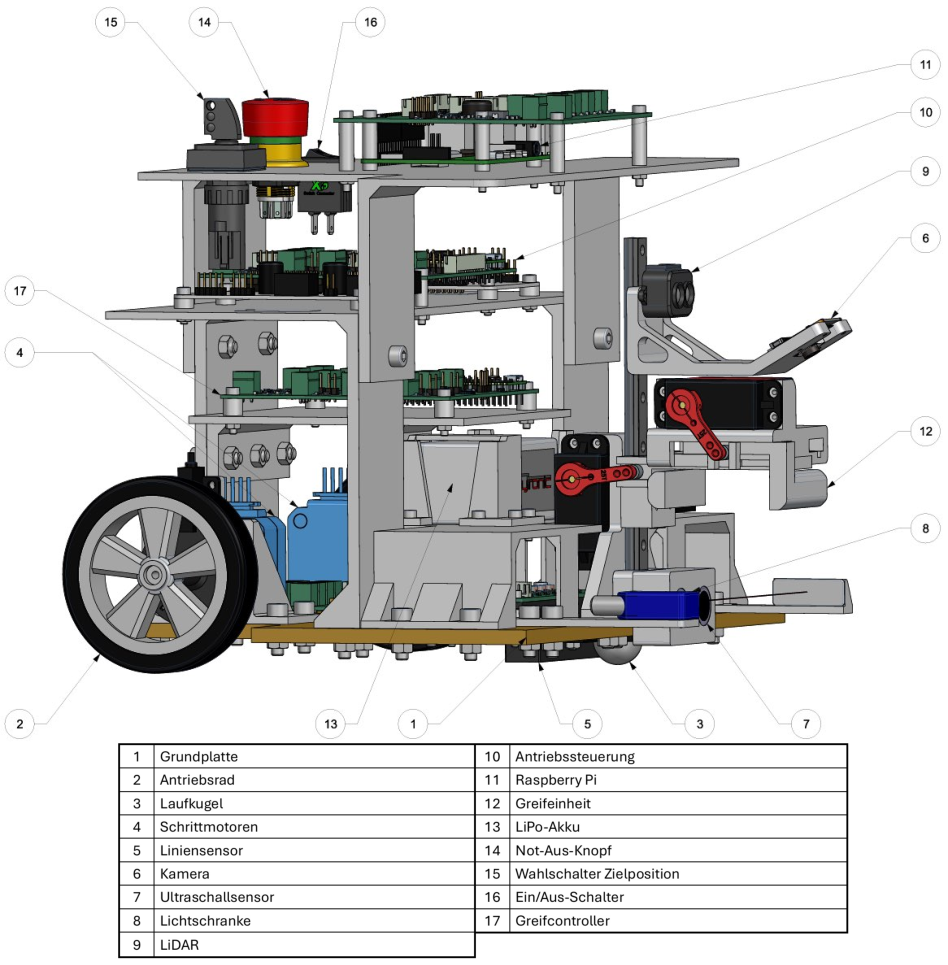
\includegraphics[width=1\textwidth]{Baugruppe_Beschriftet.pdf}
    \caption{Prototyp des Fahrzeugs mit Bildlegende in Siemens NX}~\label{fig:Baugruppe_Beschriftet}
\end{figure}

\end{document}
